\chapter{总结展望}
本项目主要实现了一个基于BLE Mesh的智能家居平台,分为BLE Mesh节点、网关端、移动端三部分,相较于现有其他智能家居其主要优势是高扩展性、高灵活性、高开放性以及低成本。对于一般用户,降低了将自己整个家庭升级为真正的智能家庭的难度;而对于具有一定技术能力的用户以及爱好者或其他智能家居厂商,则提供了一个开放的平台来更便捷地接入自己的智能设备或控制软件来实现自己的想法。

短时间内是很难做好一个项目的,重要在于后期的改进,本项目也经历了许许多多次改进(如图~\ref{fig:improvement}~),但依旧还有不足之处。例如BLE Mesh节点配对、组网的安全性还不够高,移动端不支持自动选择蓝牙或WLAN方式来对节点进行控制等。

在未来,我们将会尝试在以下方面进行改进:
\begin{itemize}
    \item 在BLE Mesh节点上接入HomeKit的BLE协议栈,并利用Mesh网络,使HomeKit用户体验可以得到显著的改善
    \item 让自动化直接在BLE Mesh网络中处理,降低网关端压力,也能提高反应速度
    \item 支持通过BLE Mesh节点三点定位判断用户位置,加强自动化能力
    \item 支持自动根据节点电量调节低功耗模式,加强节点续航能力
\end{itemize}

\begin{figure}[H]
    \centering
    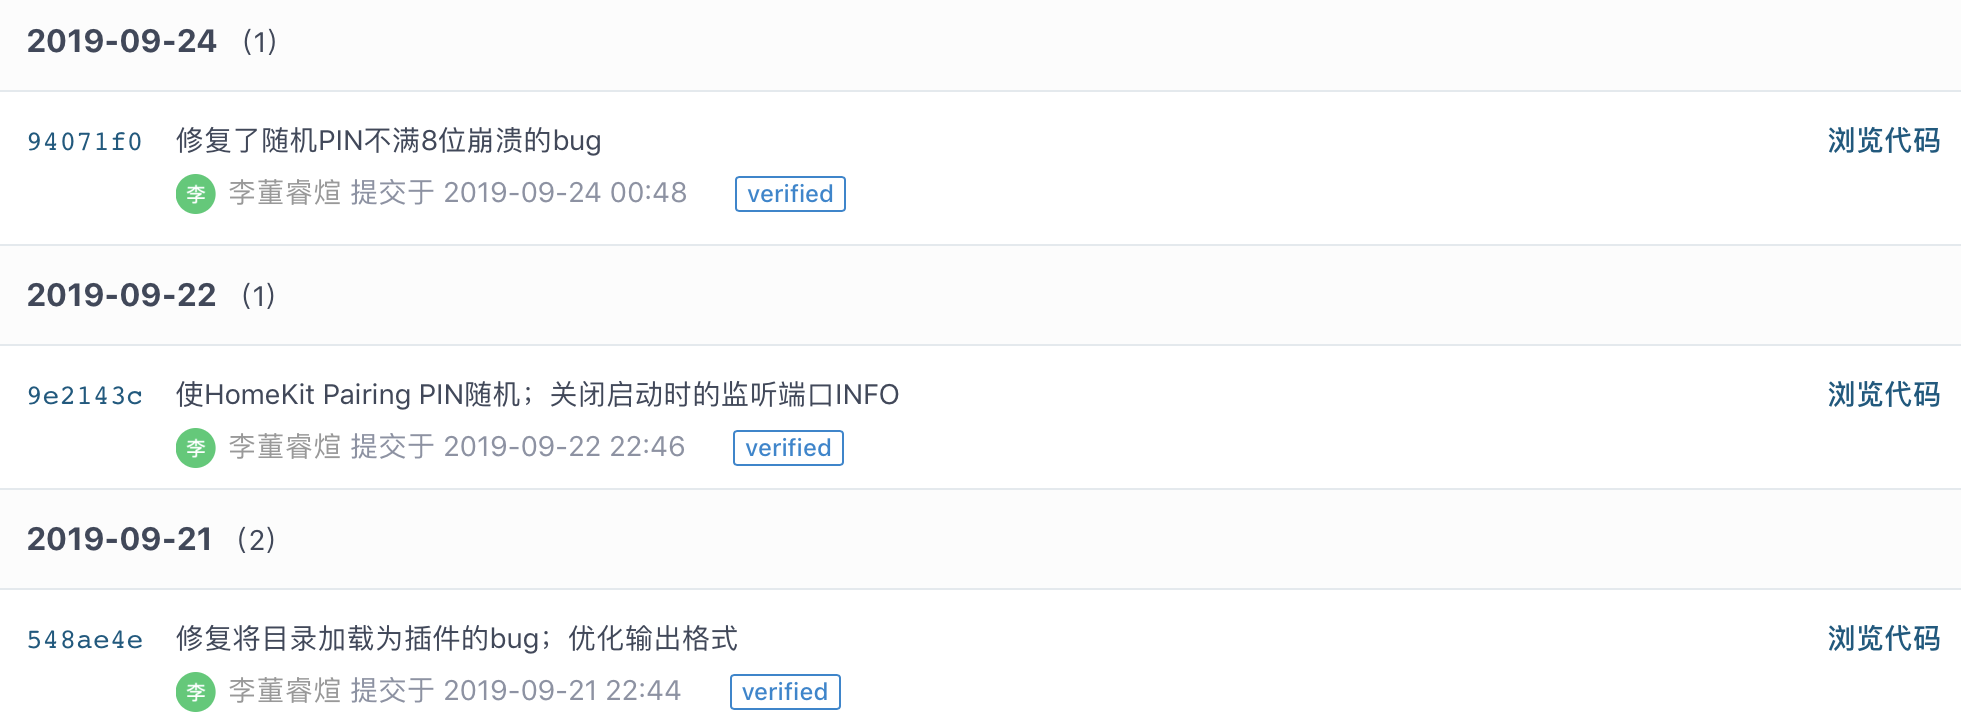
\includegraphics[width=\textwidth]{improvement.png}
    \caption{基于BLE Mesh的智能家居平台改进记录}
    \label{fig:improvement}
\end{figure}